% >>> j2l compat: xcolor / named-colour compatibility
\PassOptionsToPackage{dvipsnames}{color}
\PassOptionsToPackage{dvipsnames,svgnames,x11names,table}{xcolor}
\RequirePackage{xcolor}
\makeatletter\@namedef{ver@color.sty}{2021/01/01}\makeatother
\makeatletter\@ifundefined{providecolor}{}{%
  \providecolor{CarnationPink}{RGB}{128,128,128}
  \providecolor{Lavender}{RGB}{128,128,128}
  \providecolor{abstractcolor}{RGB}{128,128,128}
  \providecolor{rulecolor}{RGB}{128,128,128}
}\makeatother
% <<< j2l compat
\documentclass{default}
\IfFileExists{default.sty}{\usepackage{default}}{}

\IfFileExists{float.sty}{\usepackage{float}}{}
\IfFileExists{cuted.sty}{\usepackage{cuted}}{\newenvironment{strip}{\par\medskip\noindent\begin{minipage}{\linewidth}}{\end{minipage}\par\medskip}}
\makeatletter
\newcommand\jltx@wideopen{\par\addvspace{\medskipamount}\noindent}
\newcommand\jltx@wideclose{\par\addvspace{\medskipamount}}
\newenvironment{jltxspan}
  {\if@twocolumn\let\jltx@spannext\strip\else\let\jltx@spannext\jltx@wideopen\fi\jltx@spannext}
  {\if@twocolumn\let\jltx@spanend\endstrip\else\let\jltx@spanend\jltx@wideclose\fi\jltx@spanend}
\makeatother
\newcommand\JLTXaboveplacement{\par\addvspace{6pt plus 2pt minus 2pt}\noindent}
\newcommand\JLTXbelowplacement{\par\addvspace{6pt plus 2pt minus 2pt}}
\widowpenalty=10000
\clubpenalty=10000
\IfFileExists{newunicodechar.sty}{\usepackage{newunicodechar}}{\makeatletter\providecommand\newunicodechar[2]{%
  \begingroup\lccode`\~=`#1\lowercase{\endgroup\def~}{#2}%
  \catcode`#1=\active}\makeatother}
\newunicodechar{λ}{\ensuremath{\lambda}}
\newunicodechar{π}{\ensuremath{\pi}}

% >>> j2l compat: scalable Computer Modern (arbitrary font sizes)
\IfFileExists{type1cm.sty}{\usepackage{type1cm}}{}
\IfFileExists{fix-cm.sty}{\usepackage{fix-cm}}{}
% <<< j2l compat
\begin{document}
% >>> j2l compat: body-text size (+5%)
\makeatletter
\edef\JLTXbasesize{\f@size}
\@tempdimb=1.2\dimexpr\f@size pt\relax\edef\JLTXbaseskip{\strip@pt\@tempdimb}
\def\JLTXbodyscale{1.050}
\let\JLTX@normalsize\normalsize
\renewcommand\normalsize{%
  \JLTX@normalsize
  \@tempdima=\JLTXbodyscale\dimexpr\f@size pt\relax
  \@tempdimb=1.2\@tempdima
  \fontsize{\strip@pt\@tempdima}{\strip@pt\@tempdimb}\selectfont}%
\@ifundefined{@makecaption}{}{%
  \let\JLTX@makecaption\@makecaption
  \long\def\@makecaption#1#2{%
    \begingroup\fontsize{\JLTXbasesize}{\JLTXbaseskip}\selectfont
    \let\normalsize\JLTX@normalsize
    \JLTX@makecaption{#1}{#2}\endgroup}}%
\@ifundefined{thebibliography}{}{%
  \let\JLTX@thebibliography\thebibliography
  \def\thebibliography{%
    \fontsize{\JLTXbasesize}{\JLTXbaseskip}\selectfont\JLTX@thebibliography}}%
\makeatother
\normalsize
% <<< j2l compat


% Title block rendered inline (article's \maketitle forces a page break when
% preceded by other content, which pushed the whole paper to page 2).
\begin{center}
  {\LARGE\bfseries Fractional-Order Dynamics of Cardio-Respiratory Oxygen Transport: A Stable Regulator of Human Endurance and the Boundary of Chaos\par}
  \vspace{1em}
  {\normalsize Aashima Bangia$^{1}$, Rashmi Bhardwaj$^{2}$, Asokan Vasudevan$^{3}$, Naeema Darwish Khamis Al Maashari$^{4}$, Yafang Yan5 Khin Yadanar Htun$^{5}$, Email:  ORCID:$^{5}$, Email:$^{5}$, Email:  ORCID:$^{6}$, AMS Classification: 37M$^{5}$, 37M$^{5}$, 37Fxx$^{5}$, 65-XX$^{5}$, Physiological basis of the model assumptions$^{5}$, Selection of parameter values$^{5}$, leading to$^{5}$, f can be approximated through Jacobian matrix as:$^{5}$, For the system under study$^{5}$, the jacobian$^{5}$, J can be intended as:$^{5}$, Consecutively$^{5}$, Characteristic Polynomial$^{5}$, P(n) so formed is:$^{5}$, Definition: Grunwald-Letnikov Derivative$^{5}$, Binomial coefficient present in the derivative can be computed through Gamma function as:$^{5}$, Theorem: Riemann Liouville Fractional Derivative (RLFD)$^{5}$, Riemann alongwith Liouville in the year 1847 developed this derivative as:$^{5}$, having  as the well-known gamma function computed through:$^{5}$, Now$^{5}$, employing fractionalization algo for extending this fractional equation i.e.$^{5}$, as$^{5}$, the$^{5}$, Whenever$^{5}$, the RL operator reduces the equation to:$^{5}$, This is equivalent to the reduced RLFD given in equation (3).$^{5}$, Definition: Caputo Derivative for Fractional order$^{5}$, Caputo derivative is defined for fractional order$^{5}$, as:$^{5}$, Definition: Riemann-Liouville Fractional Integral(RLFI)$^{5}$, Definition: Caputo Fractional Integral$^{5}$, The integral for the order$^{5}$, defined in the sense of Caputo as:$^{5}$, having  as the well-known gamma function computed through:$^{5}$, having initial conditions:$^{5}$, where denotes the operator as defined by the Caputo as:$^{5}$, Consider the integer order general form of differential equations represented as:$^{5}$, having initial conditions:$^{5}$, which leads to the integration results derived given in [] as follows:$^{5}$, Rearranging the integration eqn. (16) as follows:$^{5}$, On employing trapezoidal rule on eqn. (16) alongwith (17)$^{5}$, it becomes$^{5}$, then eqn. (16) becomes:  such as .$^{5}$, Thus$^{5}$, Therefore$^{5}$, eqn. (20) in terms of eqn. (22) becomes:$^{5}$, And the predictor form$^{5}$, of this fractional Adams-Moulton method can be seen as:$^{5}$, This implies that as per the Adams-Moulton method is represented as:$^{5}$, Phase$^{5}$, Variation in q = [q$^{5}$, q$^{5}$, q3]$^{5}$, Variation in time period$^{5}$, t$^{5}$, Stable$^{5}$, Critical (extended model)$^{5}$, Chaotic (extended model)$^{5}$, Fractional order$^{5}$, q$^{5}$, |arg λ| min (rad)$^{5}$, qπ/$^{5}$, Regime$^{5}$, Yes$^{5}$, Stable focus$^{5}$, Yes$^{5}$, Stable focus$^{5}$, Yes$^{5}$, Stable focus$^{5}$, Yes$^{5}$, Stable focus$^{5}$, Yes$^{5}$, Stable focus$^{5}$, Yes$^{5}$, Stable focus$^{5}$, Yes$^{5}$, Stable focus$^{5}$, Table-2: Values of parameters considered in the model$^{5}$, Parameter$^{5}$, Description$^{5}$, Values$^{5}$, Mr$^{5}$, Rate of Metabolism$^{5}$, 0.01/sec$^{5}$, V$^{5}$, Maximum lung volume$^{5}$, 3600ml$^{5}$, Maximum transmission rate of molecules from lungs to bloodstream$^{5}$, 0.1/sec$^{5}$, Maximum transmission rate of molecules from bloodstream to bodycells$^{5}$, 0.7/second ()$^{5}$, Breathing-period$^{5}$, 20s inhale$^{5}$, 20s suspension$^{5}$, 20s exhale i.e.$^{5}$, 60 secs in total$^{5}$, Amount of oxygen intake under different circumstances$^{5}$, 24L/minute ()$^{5}$, Table 3: Literature studies for the kinesiology-based models$^{5}$, Year$^{5}$, Author$^{5}$, Description$^{5}$, Parameters$^{5}$, Results$^{5}$, Complexity Dynamics of Meditating Body$^{5}$, Differential model developed for the human body$^{5}$, Analysis of the human body during different meditation phases to capture varied oxygen concentration-levels$^{5}$, Teka W.W. et al$^{5}$, Spiking as well as overflowing patterns of fractional-order Izhikevich model$^{5}$, Fractional order equations developed for Izhikevich model$^{5}$, Analyzed the parameters of the fractional order apt for simulation$^{5}$, Dynamical Indicator of Human Body’s Physical Endurance$^{5}$, Fractional ordered SEQIR-based model was developed to study Coronavirus dynamics$^{5}$, Numerical simulations plotted$^{5}$, Lyapunov stability found the system to be asymptotically stable$^{5}$, Ghita M.$^{5}$, Copot D.$^{5}$, Ionescu C.M.$^{5}$, Lung cancer dynamics using fractional order impedance modeling on a mimicked lung tumor setup$^{5}$, Fractional order impedance modelling was developed to study lung tumor$^{5}$, Li Z$^{5}$, Pei Y$^{5}$, Wang Y$^{5}$, Tian Q$^{5}$, An enhanced respiratory mechanics model based on double-exponential$^{5}$, fractional calculus$^{5}$, Fractional respiratory mechanics fitted to real data$^{5}$, The hybrid model achieved significantly better results for different ventilation modes$^{5}$, Alharbi. N$^{5}$, Present study$^{5}$, Fractional Ordered Kinesiology Model$^{5}$\par}
  \vspace{0.5em}
  {\small $^{1}$ Assistant Professor, Sharda University, Greater Noida, U.P.-201310. \\ $^{2}$ Professor of Mathematics, Head, Non-Linear Dynamics Research Lab, \\ $^{3}$ Faculty of Business and Communications, INTI International University, Negeri Sembilan 71800, Malaysia. \\ $^{4}$ University School of Basic and Applied Science, GGSIPU, Delhi \\ $^{5}$ This derivative is used to describe the models with complexities as RLFD becomes incompetent to deal with the intricate systems. \\ $^{6}$ Faculty of Liberal Arts, Shinawatra University, Thailand, email: email:\par}
  \vspace{0.5em}
  {\small $^{*}$ Corresponding author e-mail: 18778460649@163.com\par}
\end{center}
\vspace{1em}

\begin{abstract}
This work develops a fractional-order dynamical model of coupled cardio-respiratory oxygen transport among the lungs, the heart and bloodstream, and the body tissues, and studies the conditions under which the human body sustains or loses stable oxygen regulation during sustained effort. The three-compartment system is formulated with Caputo fractional derivatives of order q, so that physiological memory arising from delayed oxygen uptake, circulatory transport lags, and gradual tissue utilisation is represented intrinsically rather than through added delay terms. The equilibrium structure is derived, and the associated Jacobian matrix is obtained in closed form as a real, non-symmetric operator. Local stability is established rigorously using the Matignon criterion appropriate to fractional-order systems: at the physiological operating point the eigenvalues give a minimum argument of 1.605 radians, yielding a critical order of 1.02, so the regulated state is a stable focus for every admissible order between zero and one. This analytical result is confirmed numerically by the largest Lyapunov exponent, computed with a variational method validated on the classical Lorenz system, which returns a value of -0.10 independent of the initial condition. The model therefore describes a robustly self-regulating oxygen-transport system, and this stable regime is interpreted as the dynamical basis of endurance. A physiologically motivated extension in which the cardiac response gain is separated from and exceeds the pulmonary transfer coefficient and the metabolic dissipation is raised to realistic levels undergoes a genuine transition to chaotic dynamics, offering a candidate description of cardio-respiratory dysregulation and fatigue. Notably, stronger memory (a lower fractional order) suppresses this chaos, indicating that the fractional formulation enhances the robustness of the regulated endurance state. A parameter-sensitivity analysis confirms that stability persists across the physiological ranges of the transport, breathing, and metabolic parameters. The findings connect fractional-order nonlinear dynamics to measurable endurance and recovery in sports science, physiotherapy, and cardio-respiratory health monitoring. Numerical simulations employ a fractional Adams–Bashforth–Moulton (ABM) scheme.
\end{abstract}

\noindent\textbf{Keywords:} Caputo fractional derivative, Cardio-respiratory coupling, Chaos, Largest Lyapunov exponent, Oxygen transport, Fractional order Differential Equations (FODE), Fractional order Modelling, Adam Bashforth Moulton (ABM)
\vspace{1em}

\par\medskip\noindent {\large\bfseries Conclusions\par}\smallskip

From this case-study, most importantly the relation between physical activities, exercises, postures health and happiness can be seen as mutually exclusively through important components such as Heart, Lungs and Cells/Tissues in the body is studied using Lyapunov and phase space analysis numerically simulated on MATLAB. The nonlinear differential model determines change in concentration for oxygen during musculoskeletal physical activities based on two major components heart and energy utilized by the Adenosine triphosphate (ATP) molecules using the compartment model of breath function. Model utilizes non-linear model equalities which are with respect to time at constant rate of metabolism. The phase diagram of the setup has been analyzed for the behavioral study of the equilibrium (fixed) point with the nature of that point. Eigen-system leads to phase space diagram studied the regular and chaotic behavior. The fractional order values of q=[q1, q2, q3] for the ‘LHB’ model vary from 0\textless{}q\textless{}0.25 for stable case, 0.25\textless{}q\textless{}0.5 for critical case and have values 0.5\textless{}q\textless{}1 for the chaotic phase. Thus, it is recommended that for extensive exercising and to avoid collapsing, primarily the breath function should be boosted so that the person can hold their breath for a comparatively longer period. This will in turn boost the stamina as more and more of ATP molecules will be formed and utilized.

In practical terms, the stable regulated regime provides a candidate quantitative marker of endurance: the stability margin of the oxygen-transport dynamics could be used to characterise cardio-respiratory fitness, to monitor recovery in physiotherapy, and to flag early dysregulation in health monitoring. The principal limitations are the single-subject parameterisation, the reliance on literature-based rather than individually measured parameters, and the idealised three-compartment structure; the chaotic extension, though physiologically motivated, remains to be tested against clinical data. Future work will pursue individual calibration against measured oxygen-uptake data, extension to time-varying workload, and experimental testing of the predicted stabilising role of physiological memory.

\par\medskip\noindent {\large\bfseries Acknowledgement\par}\smallskip

\JLTXaboveplacement \begin{jltxspan}%
\noindent\begin{minipage}{\linewidth}%
\centering
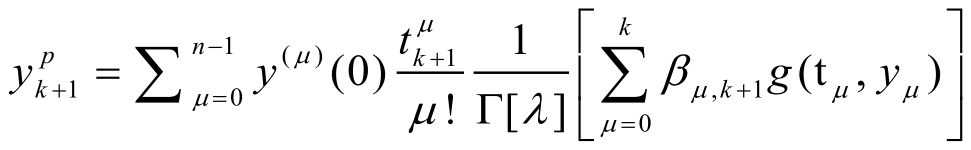
\includegraphics[width=\linewidth,height=0.3\textheight,keepaspectratio]{media/office_obj_63.png}
\label{fig:office63}%
\end{minipage}%
\end{jltxspan}\JLTXbelowplacement 

\JLTXaboveplacement \begin{jltxspan}%
\noindent\begin{minipage}{\linewidth}%
\centering
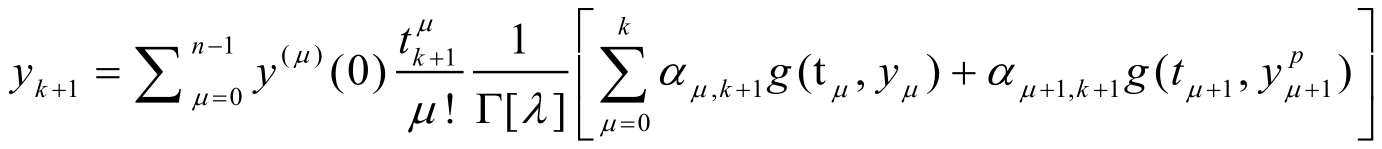
\includegraphics[width=\linewidth,height=0.3\textheight,keepaspectratio]{media/office_obj_62.png}
\label{fig:office62}%
\end{minipage}%
\end{jltxspan}\JLTXbelowplacement 

\JLTXaboveplacement \begin{jltxspan}%
\noindent\begin{minipage}{\linewidth}%
\centering
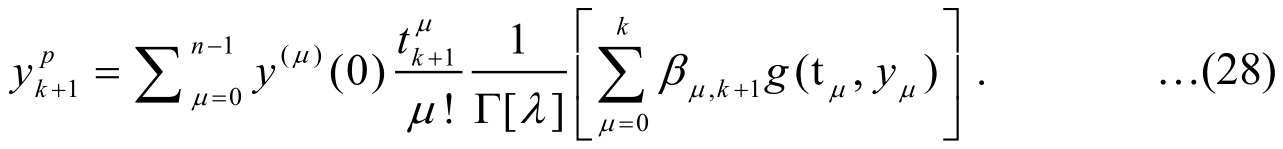
\includegraphics[width=\linewidth,height=0.3\textheight,keepaspectratio]{media/office_obj_61.png}
\label{fig:office61}%
\end{minipage}%
\end{jltxspan}\JLTXbelowplacement 

\JLTXaboveplacement \begin{jltxspan}%
\noindent\begin{minipage}{\linewidth}%
\centering
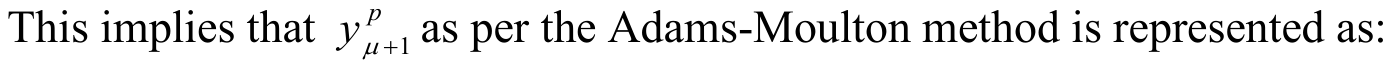
\includegraphics[width=\linewidth,height=0.3\textheight,keepaspectratio]{media/office_obj_60.png}
\label{fig:office60}%
\end{minipage}%
\end{jltxspan}\JLTXbelowplacement 

\JLTXaboveplacement \begin{jltxspan}%
\noindent\begin{minipage}{\linewidth}%
\centering
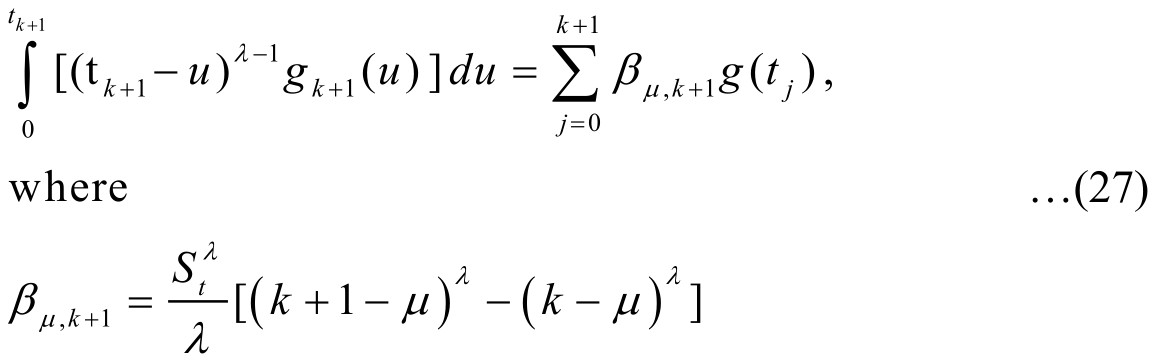
\includegraphics[width=\linewidth,height=0.3\textheight,keepaspectratio]{media/office_obj_59.png}
\label{fig:office59}%
\end{minipage}%
\end{jltxspan}\JLTXbelowplacement 

\JLTXaboveplacement \begin{jltxspan}%
\noindent\begin{minipage}{\linewidth}%
\centering
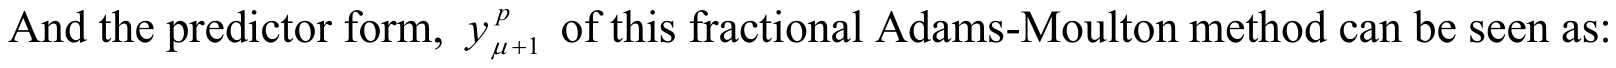
\includegraphics[width=\linewidth,height=0.3\textheight,keepaspectratio]{media/office_obj_58.png}
\label{fig:office58}%
\end{minipage}%
\end{jltxspan}\JLTXbelowplacement 

\JLTXaboveplacement \begin{jltxspan}%
\noindent\begin{minipage}{\linewidth}%
\centering
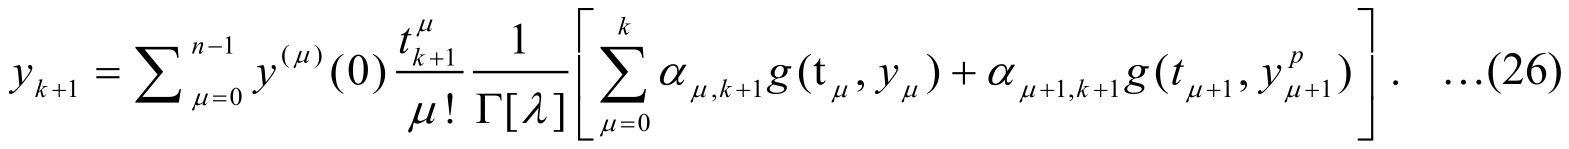
\includegraphics[width=\linewidth,height=0.3\textheight,keepaspectratio]{media/office_obj_57.png}
\label{fig:office57}%
\end{minipage}%
\end{jltxspan}\JLTXbelowplacement 

\JLTXaboveplacement \begin{jltxspan}%
\noindent\begin{minipage}{\linewidth}%
\centering
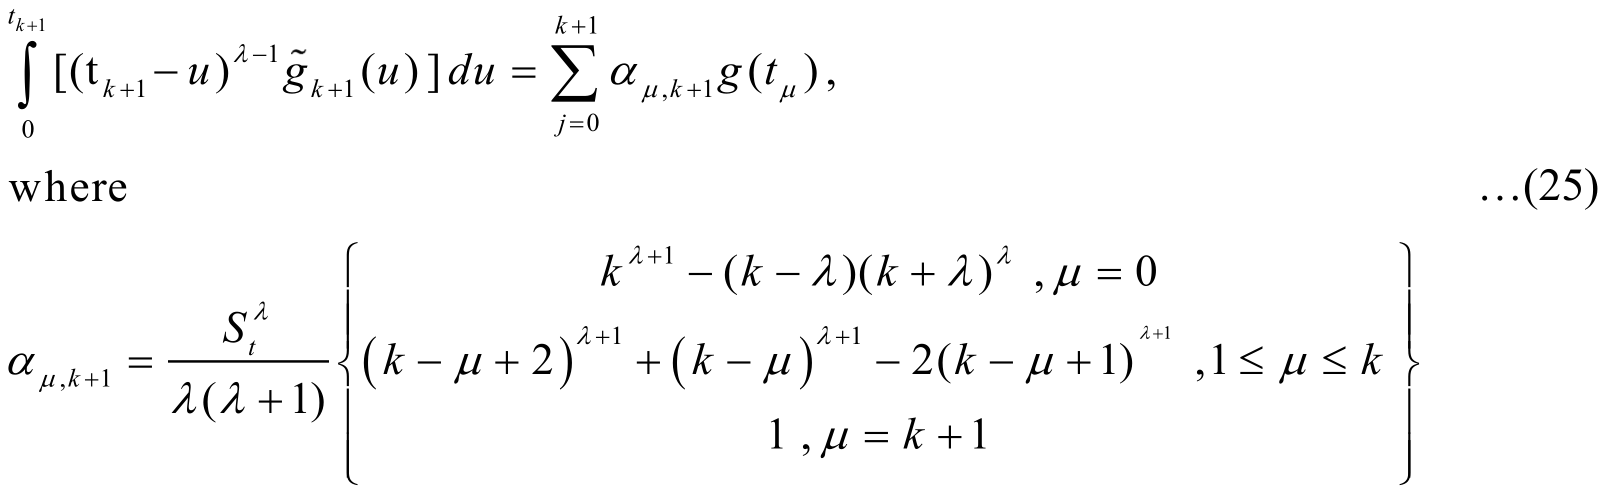
\includegraphics[width=\linewidth,height=0.3\textheight,keepaspectratio]{media/office_obj_56.png}
\label{fig:office56}%
\end{minipage}%
\end{jltxspan}\JLTXbelowplacement 

\JLTXaboveplacement \begin{jltxspan}%
\noindent\begin{minipage}{\linewidth}%
\centering
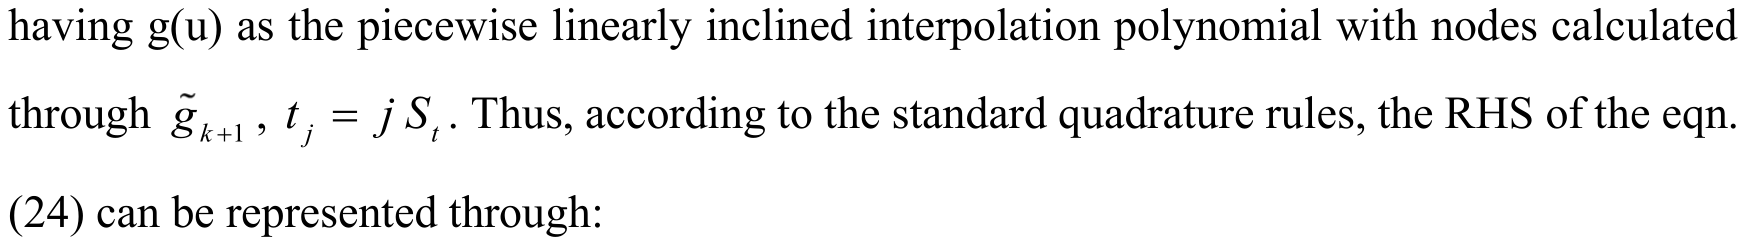
\includegraphics[width=\linewidth,height=0.3\textheight,keepaspectratio]{media/office_obj_55.png}
\label{fig:office55}%
\end{minipage}%
\end{jltxspan}\JLTXbelowplacement 

\JLTXaboveplacement \begin{jltxspan}%
\noindent\begin{minipage}{\linewidth}%
\centering
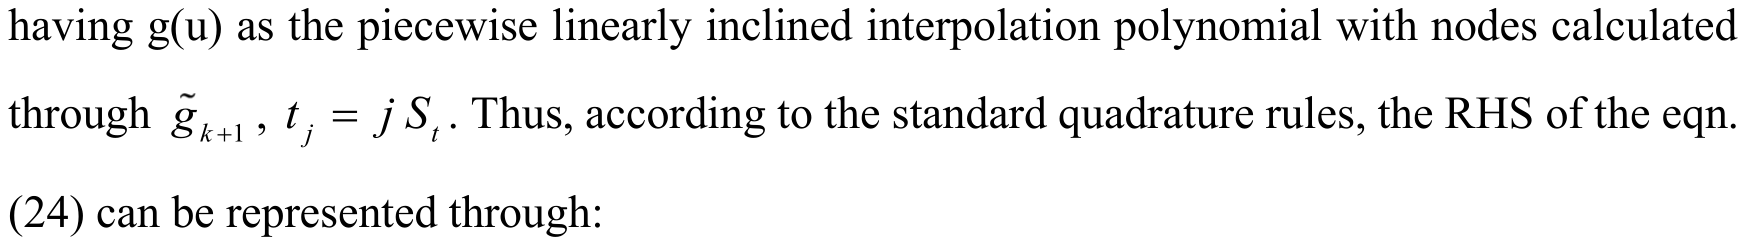
\includegraphics[width=\linewidth,height=0.3\textheight,keepaspectratio]{media/office_obj_54.png}
\label{fig:office54}%
\end{minipage}%
\end{jltxspan}\JLTXbelowplacement 

\JLTXaboveplacement \begin{jltxspan}%
\noindent\begin{minipage}{\linewidth}%
\centering
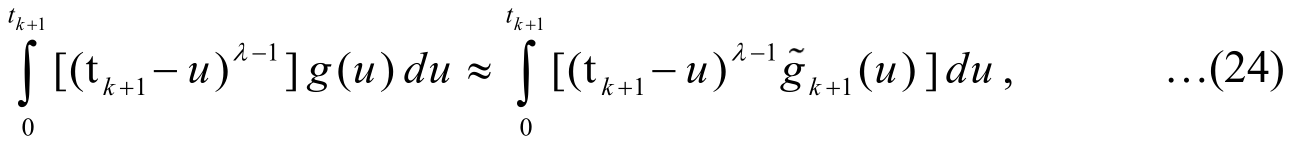
\includegraphics[width=\linewidth,height=0.3\textheight,keepaspectratio]{media/office_obj_53.png}
\label{fig:office53}%
\end{minipage}%
\end{jltxspan}\JLTXbelowplacement 

\JLTXaboveplacement \begin{jltxspan}%
\noindent\begin{minipage}{\linewidth}%
\centering
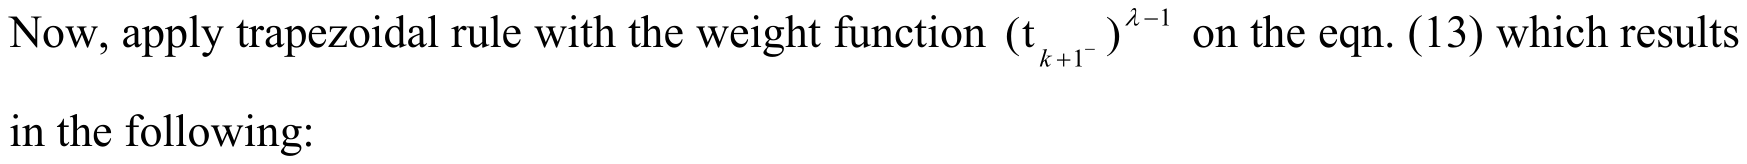
\includegraphics[width=\linewidth,height=0.3\textheight,keepaspectratio]{media/office_obj_52.png}
\label{fig:office52}%
\end{minipage}%
\end{jltxspan}\JLTXbelowplacement 

\JLTXaboveplacement \begin{jltxspan}%
\noindent\begin{minipage}{\linewidth}%
\centering
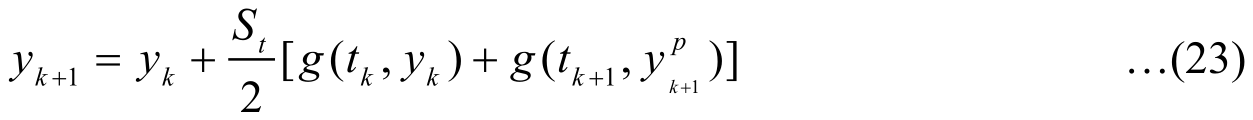
\includegraphics[width=\linewidth,height=0.3\textheight,keepaspectratio]{media/office_obj_51.png}
\label{fig:office51}%
\end{minipage}%
\end{jltxspan}\JLTXbelowplacement 

\JLTXaboveplacement \begin{jltxspan}%
\noindent\begin{minipage}{\linewidth}%
\centering
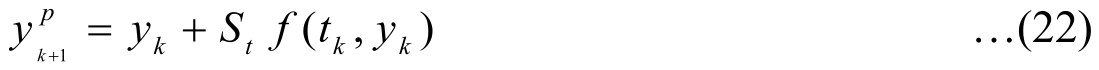
\includegraphics[width=\linewidth,height=0.3\textheight,keepaspectratio]{media/office_obj_50.png}
\label{fig:office50}%
\end{minipage}%
\end{jltxspan}\JLTXbelowplacement 

\JLTXaboveplacement \begin{jltxspan}%
\noindent\begin{minipage}{\linewidth}%
\centering
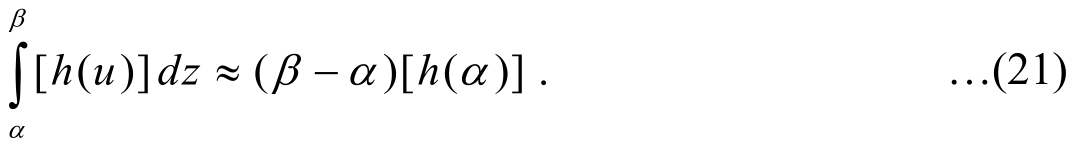
\includegraphics[width=\linewidth,height=0.3\textheight,keepaspectratio]{media/office_obj_49.png}
\label{fig:office49}%
\end{minipage}%
\end{jltxspan}\JLTXbelowplacement 

\JLTXaboveplacement \begin{jltxspan}%
\noindent\begin{minipage}{\linewidth}%
\centering
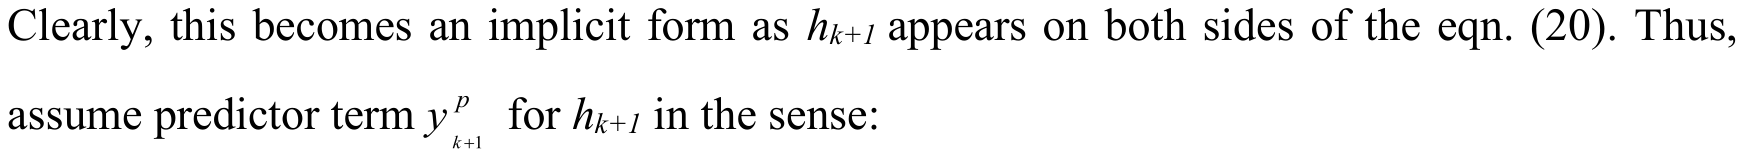
\includegraphics[width=\linewidth,height=0.3\textheight,keepaspectratio]{media/office_obj_48.png}
\label{fig:office48}%
\end{minipage}%
\end{jltxspan}\JLTXbelowplacement 

\JLTXaboveplacement \begin{jltxspan}%
\noindent\begin{minipage}{\linewidth}%
\centering
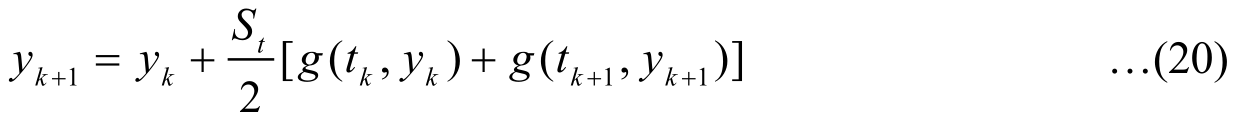
\includegraphics[width=\linewidth,height=0.3\textheight,keepaspectratio]{media/office_obj_47.png}
\label{fig:office47}%
\end{minipage}%
\end{jltxspan}\JLTXbelowplacement 

\JLTXaboveplacement \begin{jltxspan}%
\noindent\begin{minipage}{\linewidth}%
\centering
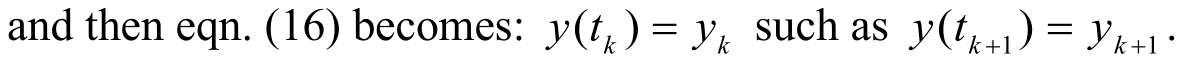
\includegraphics[width=\linewidth,height=0.3\textheight,keepaspectratio]{media/office_obj_46.png}
\label{fig:office46}%
\end{minipage}%
\end{jltxspan}\JLTXbelowplacement 

\JLTXaboveplacement \begin{jltxspan}%
\noindent\begin{minipage}{\linewidth}%
\centering
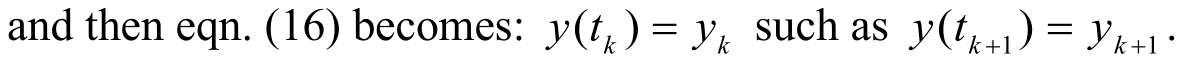
\includegraphics[width=\linewidth,height=0.3\textheight,keepaspectratio]{media/office_obj_45.png}
\label{fig:office45}%
\end{minipage}%
\end{jltxspan}\JLTXbelowplacement 

\JLTXaboveplacement \begin{jltxspan}%
\noindent\begin{minipage}{\linewidth}%
\centering
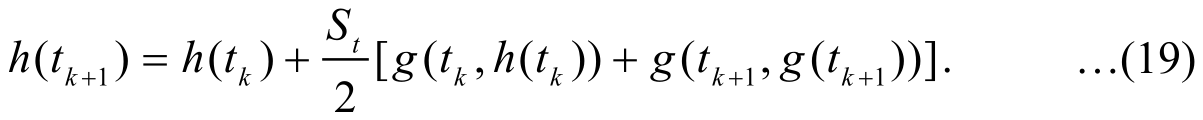
\includegraphics[width=\linewidth,height=0.3\textheight,keepaspectratio]{media/office_obj_44.png}
\label{fig:office44}%
\end{minipage}%
\end{jltxspan}\JLTXbelowplacement 

\JLTXaboveplacement \begin{jltxspan}%
\noindent\begin{minipage}{\linewidth}%
\centering
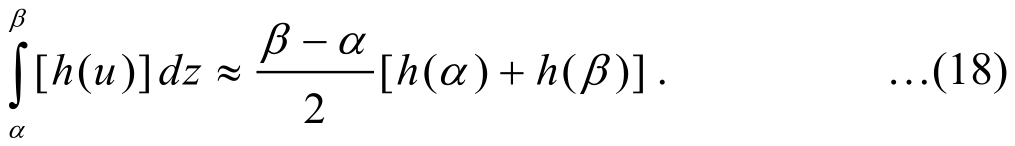
\includegraphics[width=\linewidth,height=0.3\textheight,keepaspectratio]{media/office_obj_43.png}
\label{fig:office43}%
\end{minipage}%
\end{jltxspan}\JLTXbelowplacement 

\JLTXaboveplacement \begin{jltxspan}%
\noindent\begin{minipage}{\linewidth}%
\centering
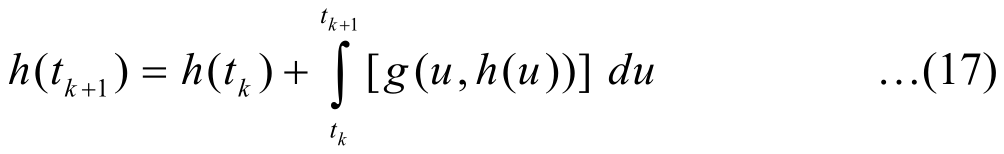
\includegraphics[width=\linewidth,height=0.3\textheight,keepaspectratio]{media/office_obj_42.png}
\label{fig:office42}%
\end{minipage}%
\end{jltxspan}\JLTXbelowplacement 

\JLTXaboveplacement \begin{jltxspan}%
\noindent\begin{minipage}{\linewidth}%
\centering
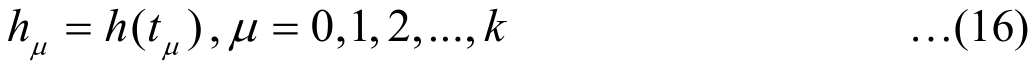
\includegraphics[width=\linewidth,height=0.3\textheight,keepaspectratio]{media/office_obj_41.png}
\label{fig:office41}%
\end{minipage}%
\end{jltxspan}\JLTXbelowplacement 

\JLTXaboveplacement \begin{jltxspan}%
\noindent\begin{minipage}{\linewidth}%
\centering
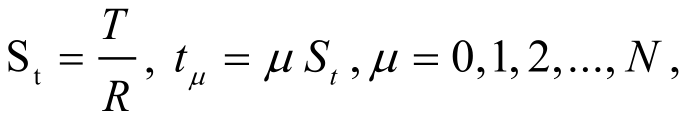
\includegraphics[width=\linewidth,height=0.3\textheight,keepaspectratio]{media/office_obj_40.png}
\label{fig:office40}%
\end{minipage}%
\end{jltxspan}\JLTXbelowplacement 

\JLTXaboveplacement \begin{jltxspan}%
\noindent\begin{minipage}{\linewidth}%
\centering
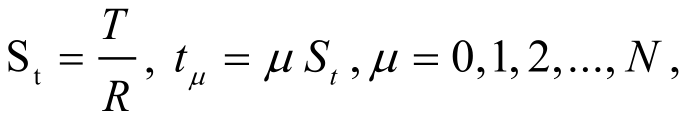
\includegraphics[width=\linewidth,height=0.3\textheight,keepaspectratio]{media/office_obj_39.png}
\label{fig:office39}%
\end{minipage}%
\end{jltxspan}\JLTXbelowplacement 

\JLTXaboveplacement \begin{jltxspan}%
\noindent\begin{minipage}{\linewidth}%
\centering
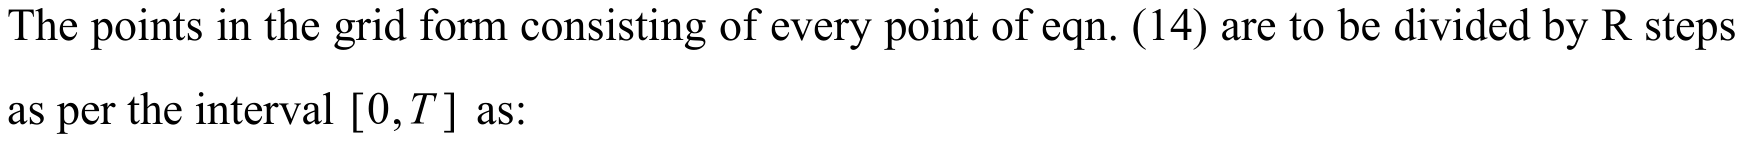
\includegraphics[width=\linewidth,height=0.3\textheight,keepaspectratio]{media/office_obj_38.png}
\label{fig:office38}%
\end{minipage}%
\end{jltxspan}\JLTXbelowplacement 

\JLTXaboveplacement \begin{jltxspan}%
\noindent\begin{minipage}{\linewidth}%
\centering
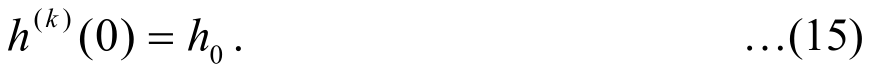
\includegraphics[width=\linewidth,height=0.3\textheight,keepaspectratio]{media/office_obj_37.png}
\label{fig:office37}%
\end{minipage}%
\end{jltxspan}\JLTXbelowplacement 

\JLTXaboveplacement \begin{jltxspan}%
\noindent\begin{minipage}{\linewidth}%
\centering
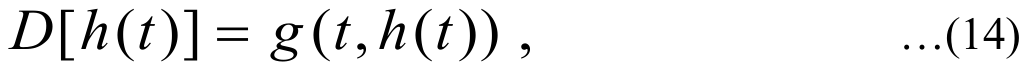
\includegraphics[width=\linewidth,height=0.3\textheight,keepaspectratio]{media/office_obj_36.png}
\label{fig:office36}%
\end{minipage}%
\end{jltxspan}\JLTXbelowplacement 

\JLTXaboveplacement \begin{jltxspan}%
\noindent\begin{minipage}{\linewidth}%
\centering
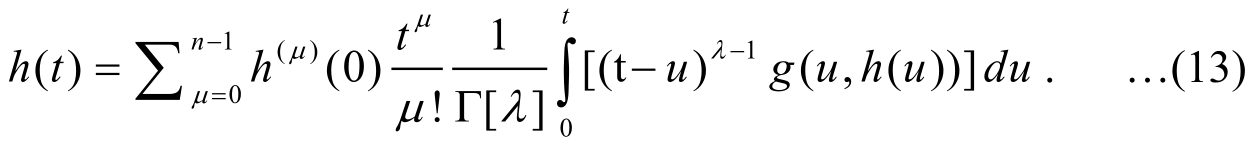
\includegraphics[width=\linewidth,height=0.3\textheight,keepaspectratio]{media/office_obj_35.png}
\label{fig:office35}%
\end{minipage}%
\end{jltxspan}\JLTXbelowplacement 

\JLTXaboveplacement \begin{jltxspan}%
\noindent\begin{minipage}{\linewidth}%
\centering
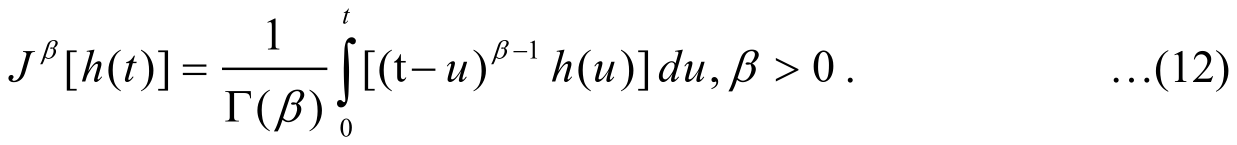
\includegraphics[width=\linewidth,height=0.3\textheight,keepaspectratio]{media/office_obj_34.png}
\label{fig:office34}%
\end{minipage}%
\end{jltxspan}\JLTXbelowplacement 

\JLTXaboveplacement \begin{jltxspan}%
\noindent\begin{minipage}{\linewidth}%
\centering
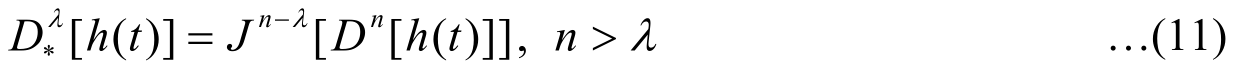
\includegraphics[width=\linewidth,height=0.3\textheight,keepaspectratio]{media/office_obj_33.png}
\label{fig:office33}%
\end{minipage}%
\end{jltxspan}\JLTXbelowplacement 

\JLTXaboveplacement \begin{jltxspan}%
\noindent\begin{minipage}{\linewidth}%
\centering
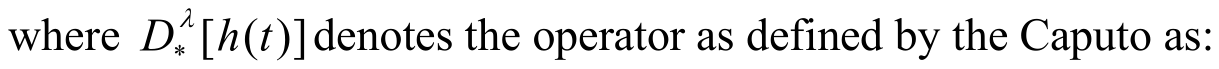
\includegraphics[width=\linewidth,height=0.3\textheight,keepaspectratio]{media/office_obj_32.png}
\label{fig:office32}%
\end{minipage}%
\end{jltxspan}\JLTXbelowplacement 

\JLTXaboveplacement \begin{jltxspan}%
\noindent\begin{minipage}{\linewidth}%
\centering
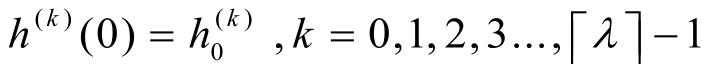
\includegraphics[width=\linewidth,height=0.3\textheight,keepaspectratio]{media/office_obj_31.png}
\label{fig:office31}%
\end{minipage}%
\end{jltxspan}\JLTXbelowplacement 

\JLTXaboveplacement \begin{jltxspan}%
\noindent\begin{minipage}{\linewidth}%
\centering
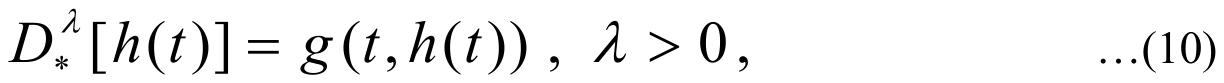
\includegraphics[width=\linewidth,height=0.3\textheight,keepaspectratio]{media/office_obj_30.png}
\label{fig:office30}%
\end{minipage}%
\end{jltxspan}\JLTXbelowplacement 

\JLTXaboveplacement \begin{jltxspan}%
\noindent\begin{minipage}{\linewidth}%
\centering
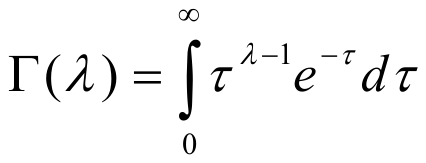
\includegraphics[width=\linewidth,height=0.3\textheight,keepaspectratio]{media/office_obj_29.png}
\label{fig:office29}%
\end{minipage}%
\end{jltxspan}\JLTXbelowplacement 

\JLTXaboveplacement \begin{jltxspan}%
\noindent\begin{minipage}{\linewidth}%
\centering
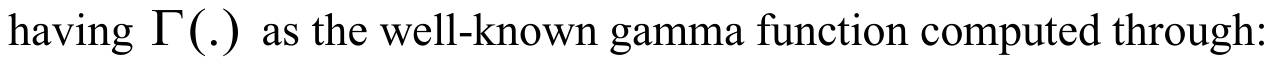
\includegraphics[width=\linewidth,height=0.3\textheight,keepaspectratio]{media/office_obj_28.png}
\label{fig:office28}%
\end{minipage}%
\end{jltxspan}\JLTXbelowplacement 

\JLTXaboveplacement \begin{jltxspan}%
\noindent\begin{minipage}{\linewidth}%
\centering
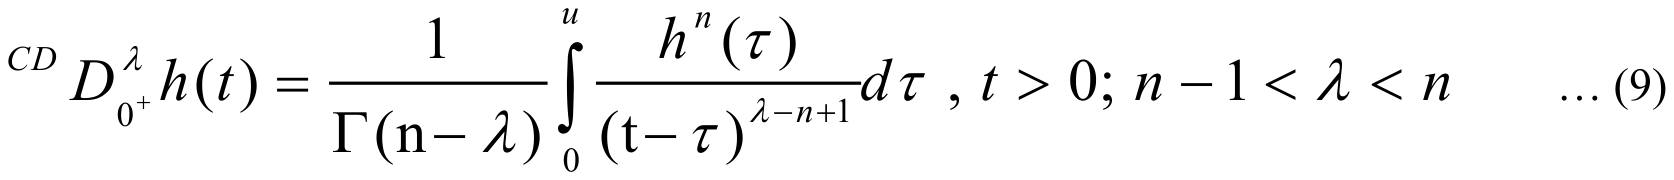
\includegraphics[width=\linewidth,height=0.3\textheight,keepaspectratio]{media/office_obj_27.png}
\label{fig:office27}%
\end{minipage}%
\end{jltxspan}\JLTXbelowplacement 

\JLTXaboveplacement \begin{jltxspan}%
\noindent\begin{minipage}{\linewidth}%
\centering
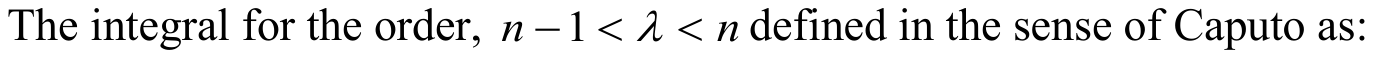
\includegraphics[width=\linewidth,height=0.3\textheight,keepaspectratio]{media/office_obj_26.png}
\label{fig:office26}%
\end{minipage}%
\end{jltxspan}\JLTXbelowplacement 

\JLTXaboveplacement \begin{jltxspan}%
\noindent\begin{minipage}{\linewidth}%
\centering
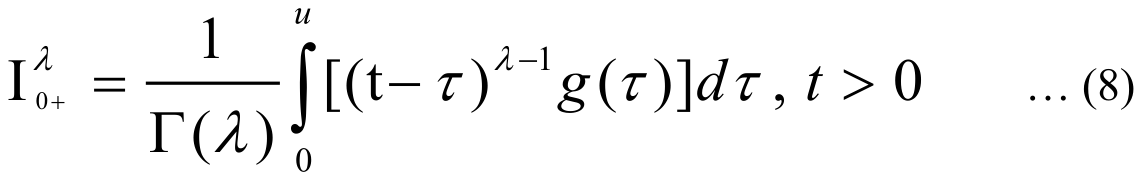
\includegraphics[width=\linewidth,height=0.3\textheight,keepaspectratio]{media/office_obj_25.png}
\label{fig:office25}%
\end{minipage}%
\end{jltxspan}\JLTXbelowplacement 

\JLTXaboveplacement \begin{jltxspan}%
\noindent\begin{minipage}{\linewidth}%
\centering
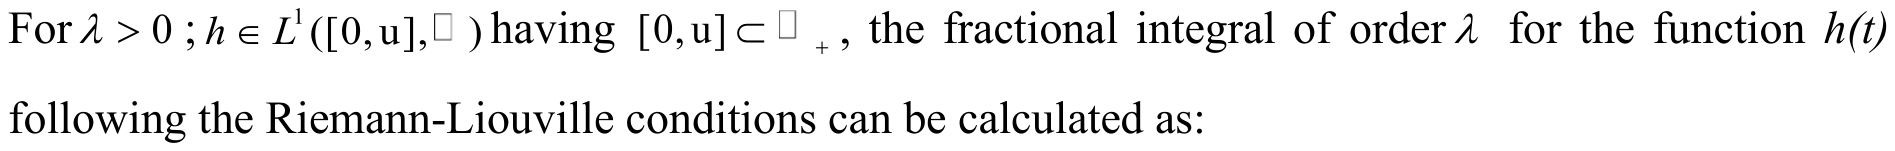
\includegraphics[width=\linewidth,height=0.3\textheight,keepaspectratio]{media/office_obj_24.png}
\label{fig:office24}%
\end{minipage}%
\end{jltxspan}\JLTXbelowplacement 

\JLTXaboveplacement \begin{jltxspan}%
\noindent\begin{minipage}{\linewidth}%
\centering
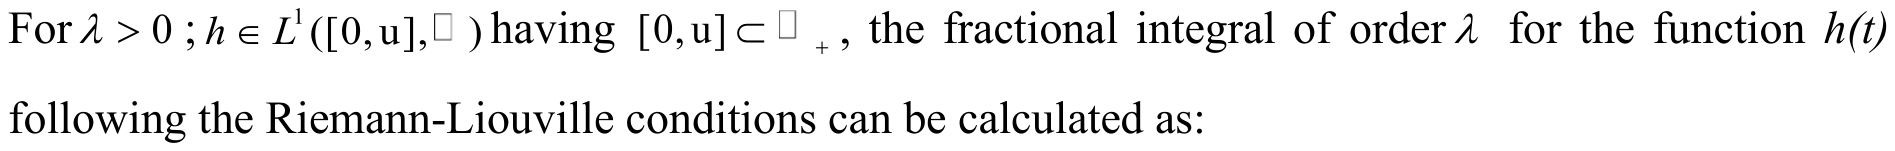
\includegraphics[width=\linewidth,height=0.3\textheight,keepaspectratio]{media/office_obj_23.png}
\label{fig:office23}%
\end{minipage}%
\end{jltxspan}\JLTXbelowplacement 

\JLTXaboveplacement \begin{jltxspan}%
\noindent\begin{minipage}{\linewidth}%
\centering
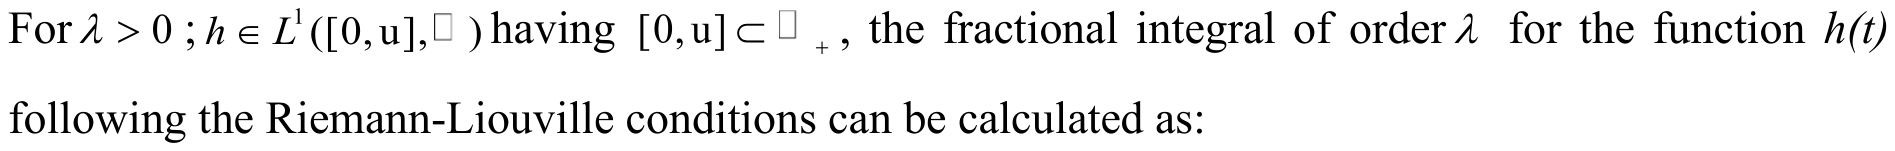
\includegraphics[width=\linewidth,height=0.3\textheight,keepaspectratio]{media/office_obj_22.png}
\label{fig:office22}%
\end{minipage}%
\end{jltxspan}\JLTXbelowplacement 

\JLTXaboveplacement \begin{jltxspan}%
\noindent\begin{minipage}{\linewidth}%
\centering
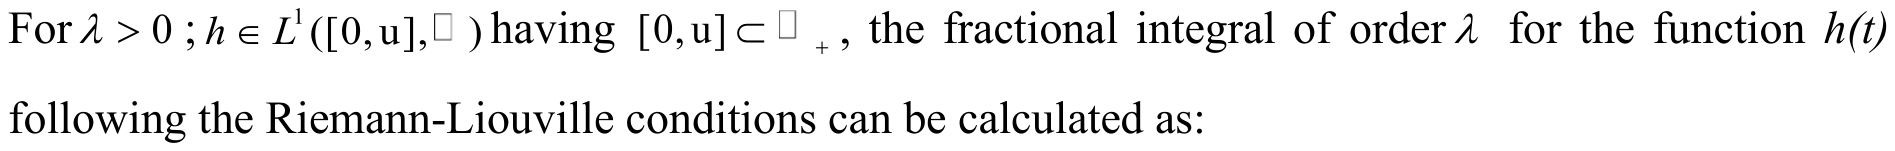
\includegraphics[width=\linewidth,height=0.3\textheight,keepaspectratio]{media/office_obj_21.png}
\label{fig:office21}%
\end{minipage}%
\end{jltxspan}\JLTXbelowplacement 

\JLTXaboveplacement \begin{jltxspan}%
\noindent\begin{minipage}{\linewidth}%
\centering
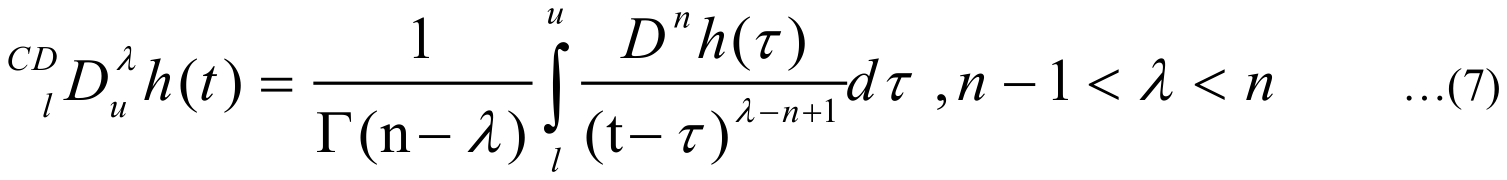
\includegraphics[width=\linewidth,height=0.3\textheight,keepaspectratio]{media/office_obj_20.png}
\label{fig:office20}%
\end{minipage}%
\end{jltxspan}\JLTXbelowplacement 

\JLTXaboveplacement \begin{jltxspan}%
\noindent\begin{minipage}{\linewidth}%
\centering
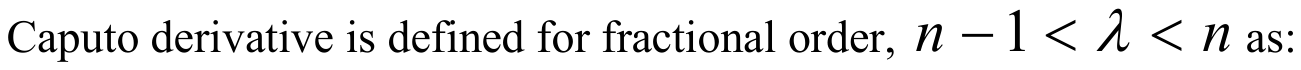
\includegraphics[width=\linewidth,height=0.3\textheight,keepaspectratio]{media/office_obj_19.png}
\label{fig:office19}%
\end{minipage}%
\end{jltxspan}\JLTXbelowplacement 

\JLTXaboveplacement \begin{jltxspan}%
\noindent\begin{minipage}{\linewidth}%
\centering
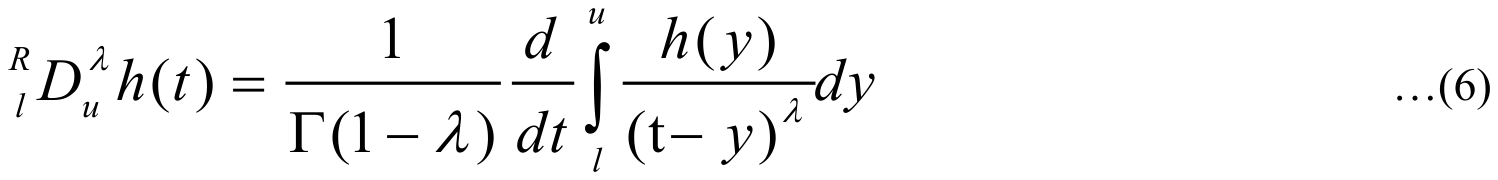
\includegraphics[width=\linewidth,height=0.3\textheight,keepaspectratio]{media/office_obj_18.png}
\label{fig:office18}%
\end{minipage}%
\end{jltxspan}\JLTXbelowplacement 

\JLTXaboveplacement \begin{jltxspan}%
\noindent\begin{minipage}{\linewidth}%
\centering
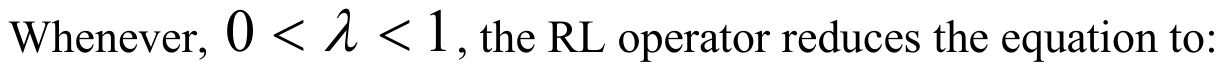
\includegraphics[width=\linewidth,height=0.3\textheight,keepaspectratio]{media/office_obj_17.png}
\label{fig:office17}%
\end{minipage}%
\end{jltxspan}\JLTXbelowplacement 

\JLTXaboveplacement \begin{jltxspan}%
\noindent\begin{minipage}{\linewidth}%
\centering
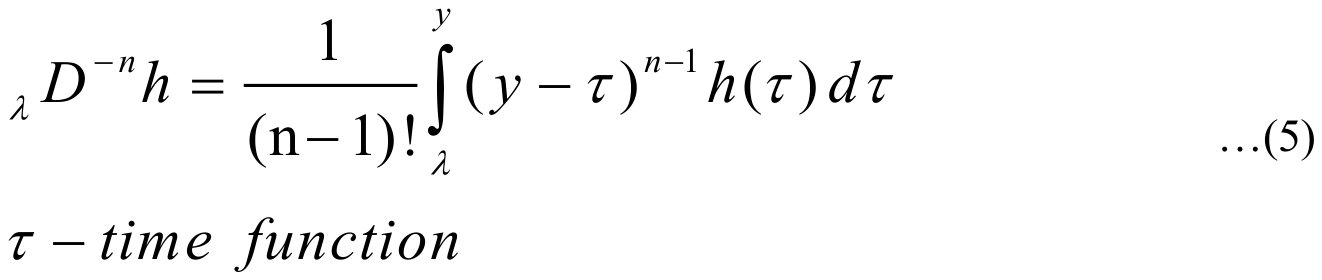
\includegraphics[width=\linewidth,height=0.3\textheight,keepaspectratio]{media/office_obj_16.png}
\label{fig:office16}%
\end{minipage}%
\end{jltxspan}\JLTXbelowplacement 

\JLTXaboveplacement \begin{jltxspan}%
\noindent\begin{minipage}{\linewidth}%
\centering
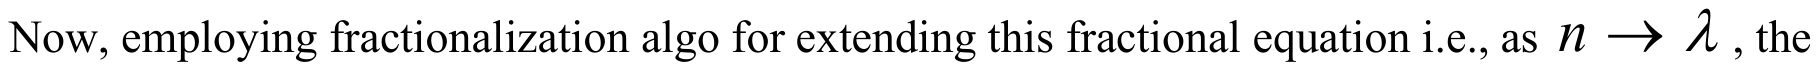
\includegraphics[width=\linewidth,height=0.3\textheight,keepaspectratio]{media/office_obj_15.png}
\label{fig:office15}%
\end{minipage}%
\end{jltxspan}\JLTXbelowplacement 

\JLTXaboveplacement \begin{jltxspan}%
\noindent\begin{minipage}{\linewidth}%
\centering
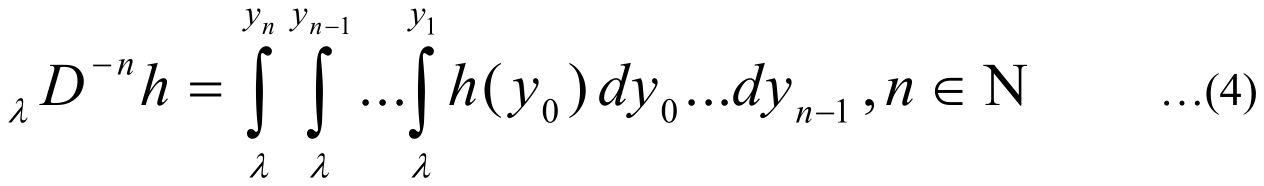
\includegraphics[width=\linewidth,height=0.3\textheight,keepaspectratio]{media/office_obj_14.png}
\label{fig:office14}%
\end{minipage}%
\end{jltxspan}\JLTXbelowplacement 

\JLTXaboveplacement \begin{jltxspan}%
\noindent\begin{minipage}{\linewidth}%
\centering
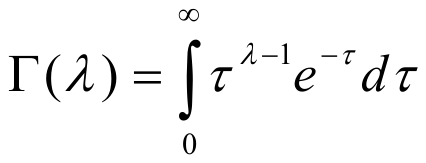
\includegraphics[width=\linewidth,height=0.3\textheight,keepaspectratio]{media/office_obj_13.png}
\label{fig:office13}%
\end{minipage}%
\end{jltxspan}\JLTXbelowplacement 

\JLTXaboveplacement \begin{jltxspan}%
\noindent\begin{minipage}{\linewidth}%
\centering
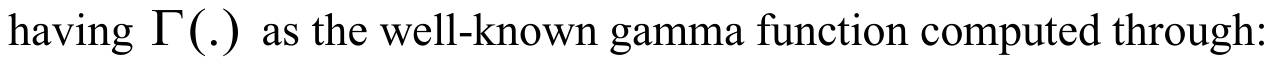
\includegraphics[width=\linewidth,height=0.3\textheight,keepaspectratio]{media/office_obj_12.png}
\label{fig:office12}%
\end{minipage}%
\end{jltxspan}\JLTXbelowplacement 

\JLTXaboveplacement \begin{figure}[H]
\centering
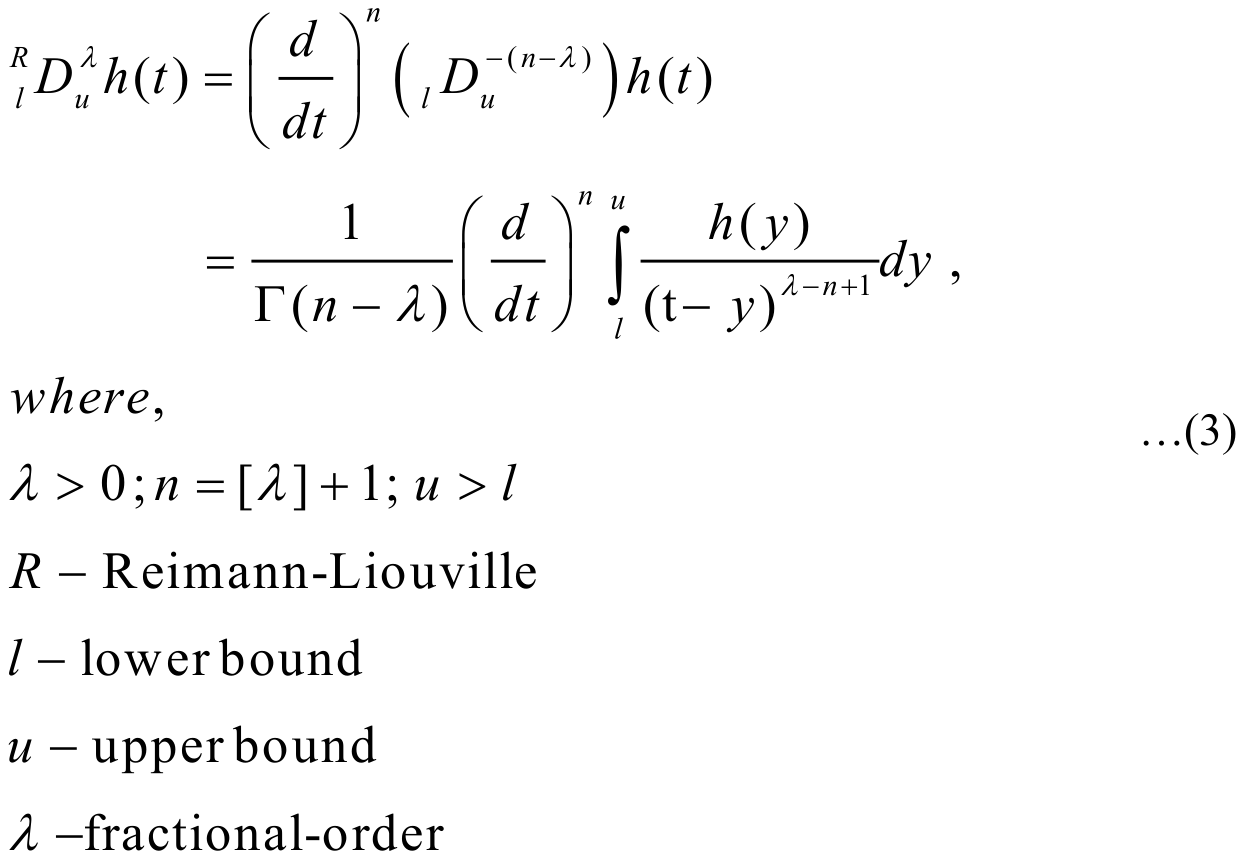
\includegraphics[width=\linewidth,height=0.3\textheight,keepaspectratio]{media/office_obj_11.png}
\label{fig:office11}
\end{figure}\JLTXbelowplacement 

\JLTXaboveplacement \begin{jltxspan}%
\noindent\begin{minipage}{\linewidth}%
\centering
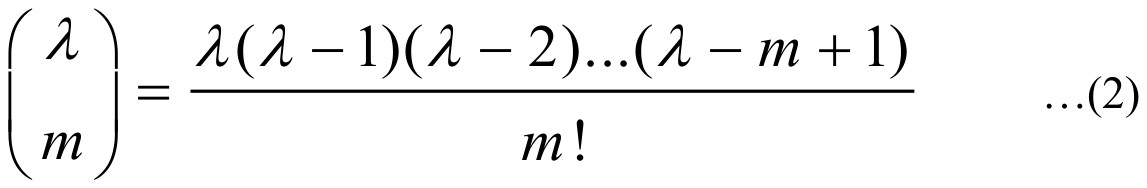
\includegraphics[width=\linewidth,height=0.3\textheight,keepaspectratio]{media/office_obj_10.png}
\label{fig:office10}%
\end{minipage}%
\end{jltxspan}\JLTXbelowplacement 

\JLTXaboveplacement \begin{jltxspan}%
\noindent\begin{minipage}{\linewidth}%
\centering
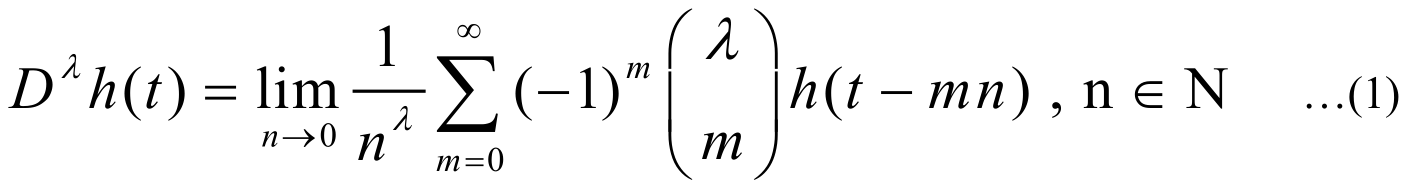
\includegraphics[width=\linewidth,height=0.3\textheight,keepaspectratio]{media/office_obj_9.png}
\label{fig:office9}%
\end{minipage}%
\end{jltxspan}\JLTXbelowplacement 

\JLTXaboveplacement \begin{jltxspan}%
\noindent\begin{minipage}{\linewidth}%
\centering
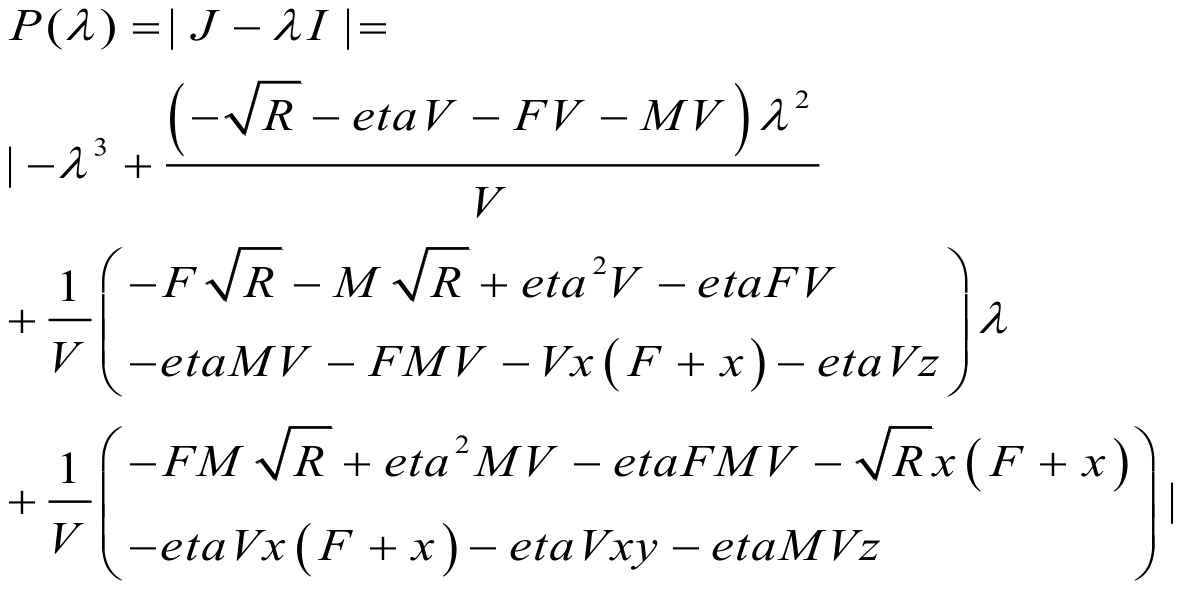
\includegraphics[width=\linewidth,height=0.3\textheight,keepaspectratio]{media/office_obj_8.png}
\label{fig:office8}%
\end{minipage}%
\end{jltxspan}\JLTXbelowplacement 

\JLTXaboveplacement \begin{jltxspan}%
\noindent\begin{minipage}{\linewidth}%
\centering

\includegraphics[width=\linewidth,height=0.3\textheight,keepaspectratio]{media/office_obj_7.png}
\label{fig:office7}%
\end{minipage}%
\end{jltxspan}\JLTXbelowplacement 

\JLTXaboveplacement \begin{figure}[H]
\centering

\includegraphics[width=\linewidth,height=0.3\textheight,keepaspectratio]{media/office_obj_6.png}
\label{fig:office6}
\end{figure}\JLTXbelowplacement 

\JLTXaboveplacement \begin{figure}[H]
\centering

\includegraphics[width=\linewidth,height=0.3\textheight,keepaspectratio]{media/office_obj_5.png}
\label{fig:office5}
\end{figure}\JLTXbelowplacement 

\JLTXaboveplacement \begin{jltxspan}%
\noindent\begin{minipage}{\linewidth}%
\centering

\includegraphics[width=\linewidth,height=0.3\textheight,keepaspectratio]{media/office_obj_4.png}
\label{fig:office4}%
\end{minipage}%
\end{jltxspan}\JLTXbelowplacement 

\JLTXaboveplacement \begin{jltxspan}%
\noindent\begin{minipage}{\linewidth}%
\centering

\includegraphics[width=\linewidth,height=0.3\textheight,keepaspectratio]{media/office_obj_3.png}
\label{fig:office3}%
\end{minipage}%
\end{jltxspan}\JLTXbelowplacement 

\JLTXaboveplacement \begin{figure}[H]
\centering

\includegraphics[width=\linewidth,height=0.3\textheight,keepaspectratio]{media/office_obj_2.png}
\label{fig:office2}
\end{figure}\JLTXbelowplacement 

\JLTXaboveplacement \begin{figure}[H]
\centering

\includegraphics[width=\linewidth,height=0.3\textheight,keepaspectratio]{media/office_obj_1.png}
\label{fig:office1}
\end{figure}\JLTXbelowplacement 

All authors are thankful for their respective institutes for providing the research facilities.

Declarations

Conflict of Interest: No conflict of interest for publication of this article.

Data Availability Statement: No Data associated in the manuscript.

\begin{thebibliography}{99}
\bibitem{ref1}
Bhardwaj, R. \& Bangia, A. (2019). Dynamic Indicator for the prediction of Atmospheric Pollutants. Asian Journal of Water, Environment and Pollution. 16(4), 39-50.

\bibitem{ref2}
Bhardwaj, R. \& Bangia, A. (2016). Complexity Dynamics of Meditating Body. Indian Journal of Industrial and Applied Mathematics. 7(2), 106-116.

\bibitem{ref3}
Bhardwaj, R. \& Bangia, A. (2018). Statistical Time series Analysis of Dynamics of HIV. JNANABHA. Special Issue 48, 22-27.

\bibitem{ref4}
Bhardwaj, R. \& Bangia, A. (2020). Dynamical Forensic Inference for Malware in IoT-Based Wireless Transmissions. In K. Sharma, M. Makino, G. Shrivastava, \& B. Agarwal (Eds.) Forensic Investigations and Risk Management in Mobile and Wireless Communications. pp. 51-79.

\bibitem{ref5}
Bhardwaj R.; Bangia, A. (2021) Dynamical Indicator of Human Body’s Physical Endurance. Nepal Journal of Mathematical Sciences (NJMS), 2(1) Feb.2021, 25-35.

\bibitem{ref6}
Baskonus, H.M. and Bulut, H. (2015). On the numerical solutions of some fractional ordinary differential equations by fractional Adams-Bashforth-Moulton method. Open Mathematics, vol. 13, no. 1.

\bibitem{ref7}
Buckley J.P., Hedge A., Yates, T., Copeland, R.J., Loosemore, M., Hamer, M., Bradley, G. and Dunstan, D.W. (2015). The sedentary office: A growing case for change towards better health and productivity. British Journal of Sports Medicine. 49, 1357-1362.

\bibitem{ref8}
Bhuvaneswari V., Balachandran K. (2020). Lower Bound of Blow up Time for Three Species Cooperating Model. Journal of Applied Nonlinear Dynamics. 9(3), 391-400.

\bibitem{ref9}
Buman M.P., King A.C. (2010). Exercise as a Treatment to Enhance Sleep. American Journal of Lifestyle Medicine. 4(6), 500-514.

\bibitem{ref10}
Cobiaga R., Reartes W. (2020). Dynamic Scenario in HTLV-I Infection. Journal of Applied Nonlinear Dynamics. 9(3), 349-359.

\bibitem{ref11}
Costa A., Costantino M.L. and Fumero R. (1992). Oxygen exchange mechanisms in the human placenta: mathematical modelling and simulation. Journal of Biomedical Engineering, 14(5), 385-389.

\bibitem{ref12}
Dinas, P.C.; Koutedakis, Y and Flouris, A.D. (2011). Effects of exercise and physical activity on depression. Irish Journal of Medical Science. 180(2), 319-325.

\bibitem{ref13}
Hasan M.N, Uddin M.S., Biswas M.H.A. (2020). Interactive Effects of Disease Transmission on Predator-Prey Model. Journal of Applied Nonlinear Dynamics. 9(3), 401-413.

\bibitem{ref14}
Jaisri, G., Dayananda, G. and Saraswathi Hegde, S.C. (2011). Heart rate variability during meditation in Pranic healers. NJIRM, 2(4), 113-116.

\bibitem{ref15}
Lajmiri Z., Ghaziani R.K. (2018). Hopf-Bifurcation and stability analysis of an predator-prey system with Holling type-IV functional response. Journal of Applied Nonlinear Dynamics. 7(4), 337-348.

\bibitem{ref16}
Sharomia, O.; Gumel, A.B. (2008). Dynamical analysis of a multi-strain model of HIV in the presence of anti-retroviral drugs, J. Biol. Dyn. 2, 323-345.

\bibitem{ref17}
Sharma, S.K.; Bangia, A.; Alshehri, M.;
Bhardwaj, R. (2021). Nonlinear Dynamics for the spread of Pathogenesis of COVID-19 Pandemic. Journal of Infection and Public Health. 14(7), 817-831 Doi:

\bibitem{ref18}
Teka W.W., Upadhyay, R.K., A. Mondal (2018). Spiking and bursting patterns of fractional-order Izhikevich model. Communications in Nonlinear Science and Numerical Simulation, 56, 161-176.

\bibitem{ref19}
Vyas R., Nirupma, D. (2002). Effect of meditation on respiratory system, cardiovascular system and lipid profile. Indian Journal of Physiology and Pharmacology. 46(4), 487-491.

\bibitem{ref20}
Wodarz; D.; Levy, D.N. (2011). Effect of different modes of viral spread on the dynamics of multiply infected cells in human immune-deficiency virus infection. J. R. Soc. Interface. 8, pp. 289-300.

\bibitem{ref21}
Alharbi. N (2026) Existence, Optimal Control, and Numerical Analysis of a Caputo Fractional Model for Oxygen Saturation Regulation. Symmetry, 18(3):482. Doi:10.3390/sym18030482

\bibitem{ref22}
Li Z, Pei Y, Wang Y and Tian Q (2023) An enhanced respiratory mechanics model based on double-exponential and fractional calculus. Front. Physiol. 14:1273645. Doi: 10.3389/fphys.2023.1273645

\bibitem{ref23}
Ghita M., Copot D., Ionescu C.M. (2021) Lung cancer dynamics using fractional order impedance modeling on a mimicked lung tumor setup. J. Advanced Research, 32:61-71.

\end{thebibliography}


\end{document}
